\documentclass{article}
\usepackage{graphicx}
\usepackage{amsmath}
\usepackage{fancyhdr}
\usepackage{hyperref}
\pagestyle{fancy}
\lhead{Ali Abdollahi}
\rhead{Project 2}
\cfoot{Page \thepage}
\title{The Second Project\\\large Synapses, Neural Population,\\and Decision Making}
\begin{document}
	\maketitle
	\section{Updates on Previous LIF}
	In this project, we apply some changes on the previous LIF model, which would be explained in the following parts:
	\subsection{Random Potentials}
	In the previous part there was almost no difference between neurons in a neuron group! As we want some variation in neuronal behavior in this project, we add some noise to the resting potential, the reset potential, and the threshold. This change make neurons to spike at various times. That is a vital point, when we want to work with a network rather than a neuron!
	
	\subsection{Input bugs fixed}
	In previous model, due to the fact that the only stimulation of the neurons was the input function and there was no connections, in the `InputBehavior`, we set the neurons input. While in this version, it just changes in the mentioned behavior, and would be reset in the neuron model, right after the input changes the potential.\\
	
	This generally would have no effect, if the input behavior's order is before the synaptic behavior. Yet, it is better to make the work easier!
	\section{The synapses}
	\subsection{Dirac Delta Function}
	With delta function, each input happens in just one moment. This means each spike affect the post-synaptic neuron just in one time step. This is the simplest method to pass the spike from dendrites to the soma, although it is not very compatible with our observations from the brain.\\
	\begin{figure}[h]
		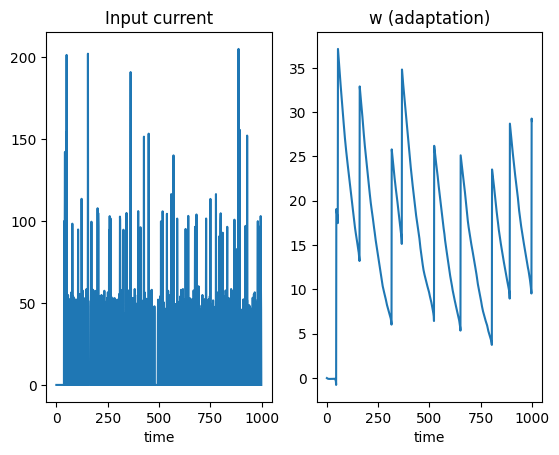
\includegraphics[width=\textwidth]{input1.png}
		\caption{\textbf{Left plot: }shows the input created by 100 pre-synaptic neurons, which they are connected to one post-synaptic neuron. \textbf{Right plot } is `w`, the parameter of adaptation.}
		\label{diracInp}
	\end{figure}
	
	For simulation, we connect 100 pre-synaptic neurons to a single neuron to investigate their effect on that. The weights were initiated randomly from a normal distribution with the mean of 50 and the standard deviation of 5 ($\sim \mathcal{N}(50, 5)$). The input of those 100 neurons is just a constant current of an amplitude of 30.
	
	In figure \ref{diracInp}, we can observe the input current, which those 100 neurons impose on one neuron. This input cause the `w` parameter to change as the right plot. It grows as inputs cause a spike in the post-synaptic neuron, and falls gradually. The voltage changes and spikes were shown in the plot \ref{diracVol}. The sub-threshold region shows how the spikes of the pre-synaptic neurons aggregated together. As there was no learning rule here and weights were random, there is no obvious spike pattern.
	
	\begin{figure}[h]
		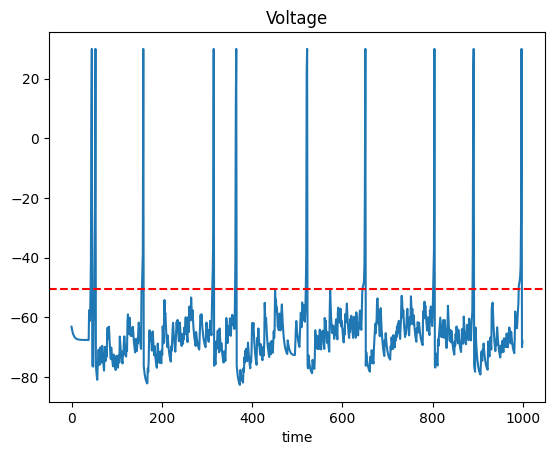
\includegraphics[width=0.8\textwidth]{voltage1.png}
		\caption{The trajectory of voltage through 1000 iterations}
		\label{diracVol}
	\end{figure}
	
	\subsection{Conductance-based Synapses}
	In delta method, each spike affect the post-synaptic neurons just in one timestamp. However, in reality, the input spikes affect the post neuron gradually, in a conductance-based manner. We can use the following formula for calculating the input current:
	
	\begin{align*}
		I_i(t) = \sum_{j} \sum_{f} &w_{ij}g\left( t-t_j^{(f)}\right)\\
		\text{Where:}\hspace*{1cm} &g(t) = g_0 + g_1 e^{-t/\tau}
	\end{align*}
	
	Where $\tau$, $g_0$, and $g_1$ are parameters. In this manner $I(t)$ decays exponentially. The above equation is simply the sum of all the exponentially-decayed-spikes of all the pre-neurons. We can calculate $\Delta G$ as follow:\\
	\begin{align*}
		\Delta g &= g_1(e^{-t/\tau} (1 - e^{1/\tau}))\\
		&= \alpha e^{-t/\tau} 
	\end{align*}
	
	Where $\alpha = g_1 (1 - e^{1/\tau})$ and $\tau$ are constants. Moreover, $g$ would be initiated to $g_{init} = g_0$. In summary, $g$ is $g_{init}$ at first. Then, it changes as $\Delta G = \alpha e^{-t/\tau}$.\\
	\subsubsection*{Comparison:}
	\begin{figure}[h]
		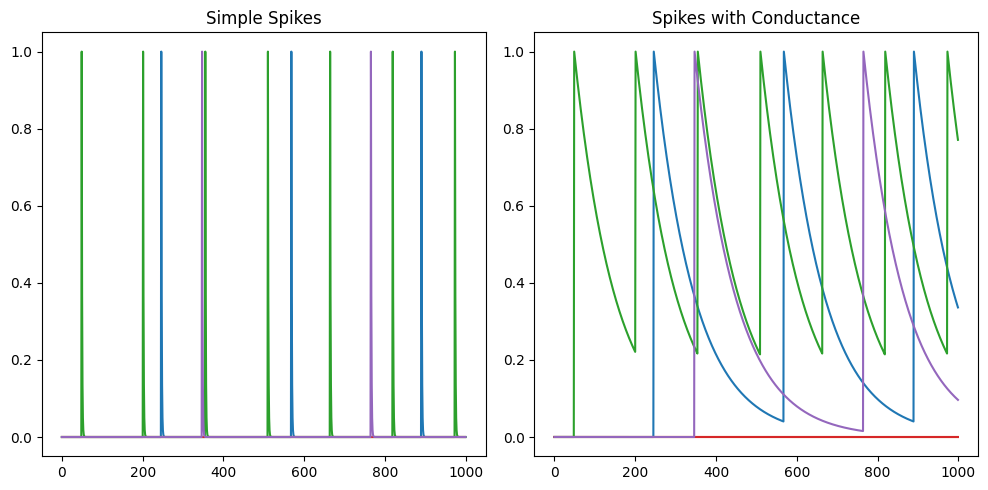
\includegraphics[width=\textwidth]{condG.png}
		\caption{A comparison between simple spikes and when we add conductivity to them. This number would be multiply by the weights and add together to construct the input. For clarity, the neurons number decreased to 5.}
		\label{condG}
	\end{figure}
	\begin{figure}
		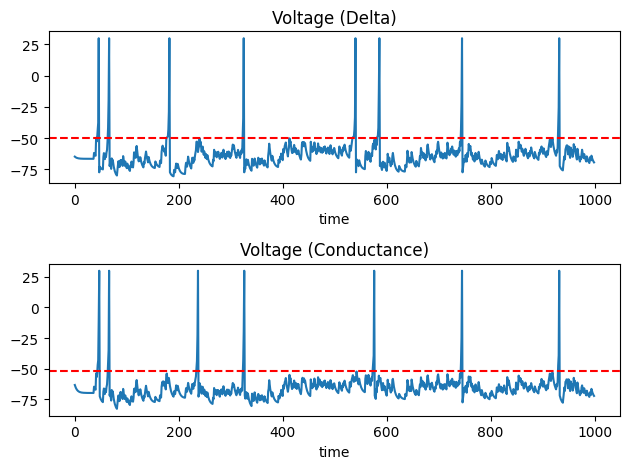
\includegraphics[width=\textwidth]{voltageComp.png}
		\caption{A comparison between voltages of two models of synapses}
		\label{volComp}
	\end{figure}
	In figure \ref{condG}, we could see a comparison between two cases. When adding conductivity to inputs, the effects of each spike remains for some time. In the figure \ref{volComp}, we can see how the voltage changes differs in two scenarios.
	
	We should also mention that although considering conductivity is more bio-plausible, it needs more computation (in delta mode, we just need to do a sum over the weights of spiked neurons. However, in this case, we also need a multiplication of 'g' and the weights)
	
	\section{Connectivity Patterns:}
	In this section, we investigate three different connectivity patterns: \textbf{1)} the full connectivity, where every neuron connects to all possible pre-synaptic neurons, \textbf{2)} random connectivity with fixed connection probability, and \textbf{3)} random connectivity with fixed number of pre-synaptic neurons.\\
	In all the states, the input is formed by 800 excitatory and 200 inhibitory pre-synaptic neurons. The input of these 1000 neurons is a constant voltage of $20A$. Moreover, both excitatory and inhibitory neuron groups have an adaptive behavior, and as we can see in all the figures \ref{fullCon}, \ref{fixProb}, and \ref{fixCount} the input has decreased over after first spikes, and stabilized from there on.
	
	\subsection{Full Connectivity}
	For a fully connected connections, there is a synapse between all the pre and post-synaptic neurons. The weights have the mean of $\frac{w_{mean}}{N}$ ($\sim \mathcal{N}(\frac{w_{mean}}{N}, \frac{w_{mu}}{N})$). \\
	In figure \ref{fullCon}, 
	
	\begin{figure}[h]
		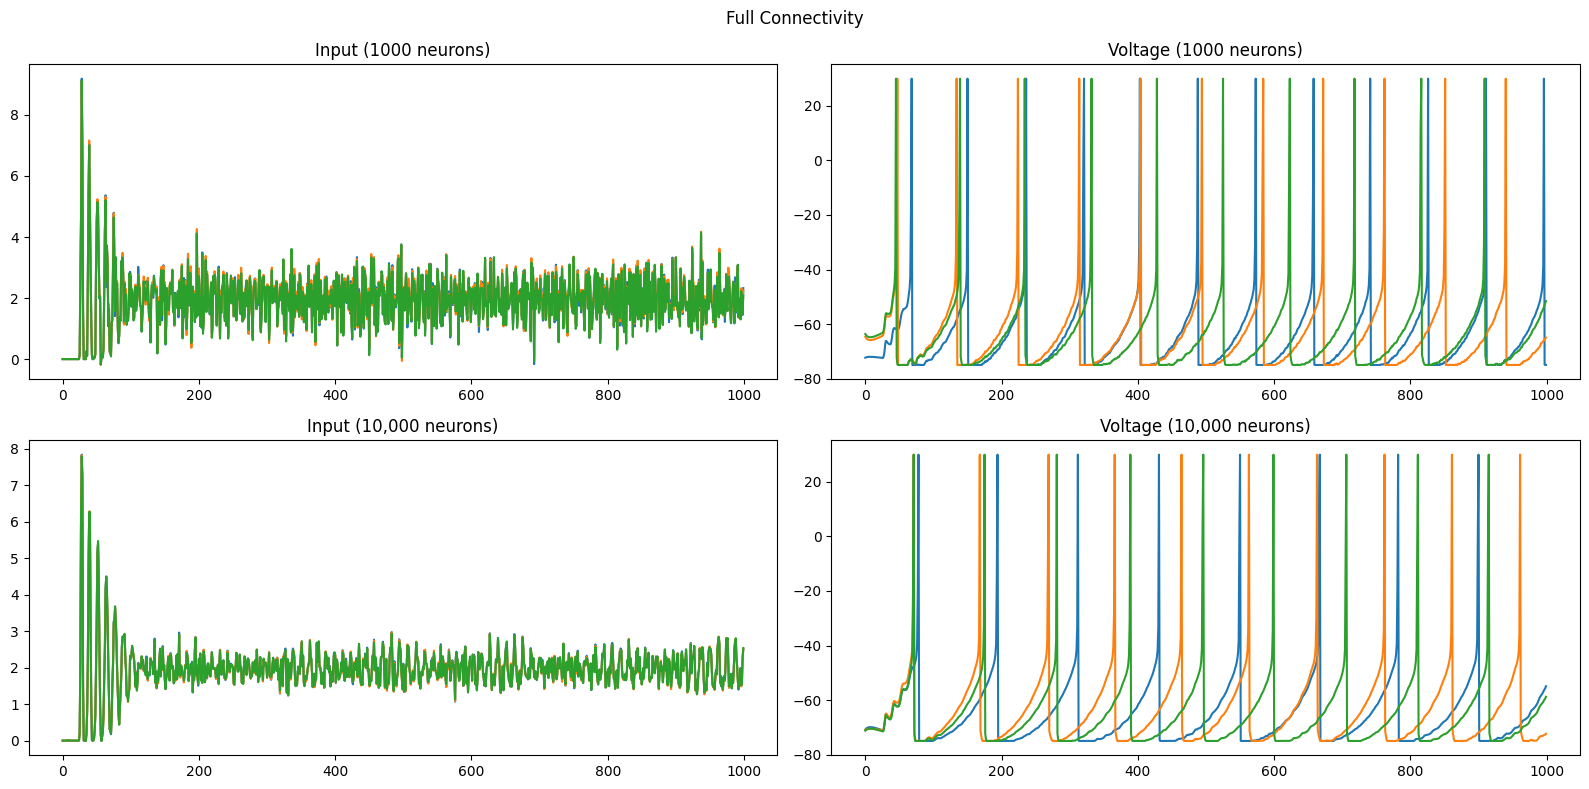
\includegraphics[width=1.2\textwidth]{fullCon.png}
		\caption{The model of full connectivity}
		\label{fullCon}
	\end{figure}
	\subsection{Fixed Probability Connectivity}
	In this case, each possible connection emerges with a fixed probability (in our model 10\%). Although, this model is almost bio-plausible, there are some problems when we scale up our model. This problem is due to the fact that the number of synapses would not increase with the ratio of growth of the neurons. For example, while in most studies, they use 10\% probability of connectivity, it does not make sense to use 10 times more synapses when we scale up the neurons 10 folds!
	
	\begin{figure}[h]
		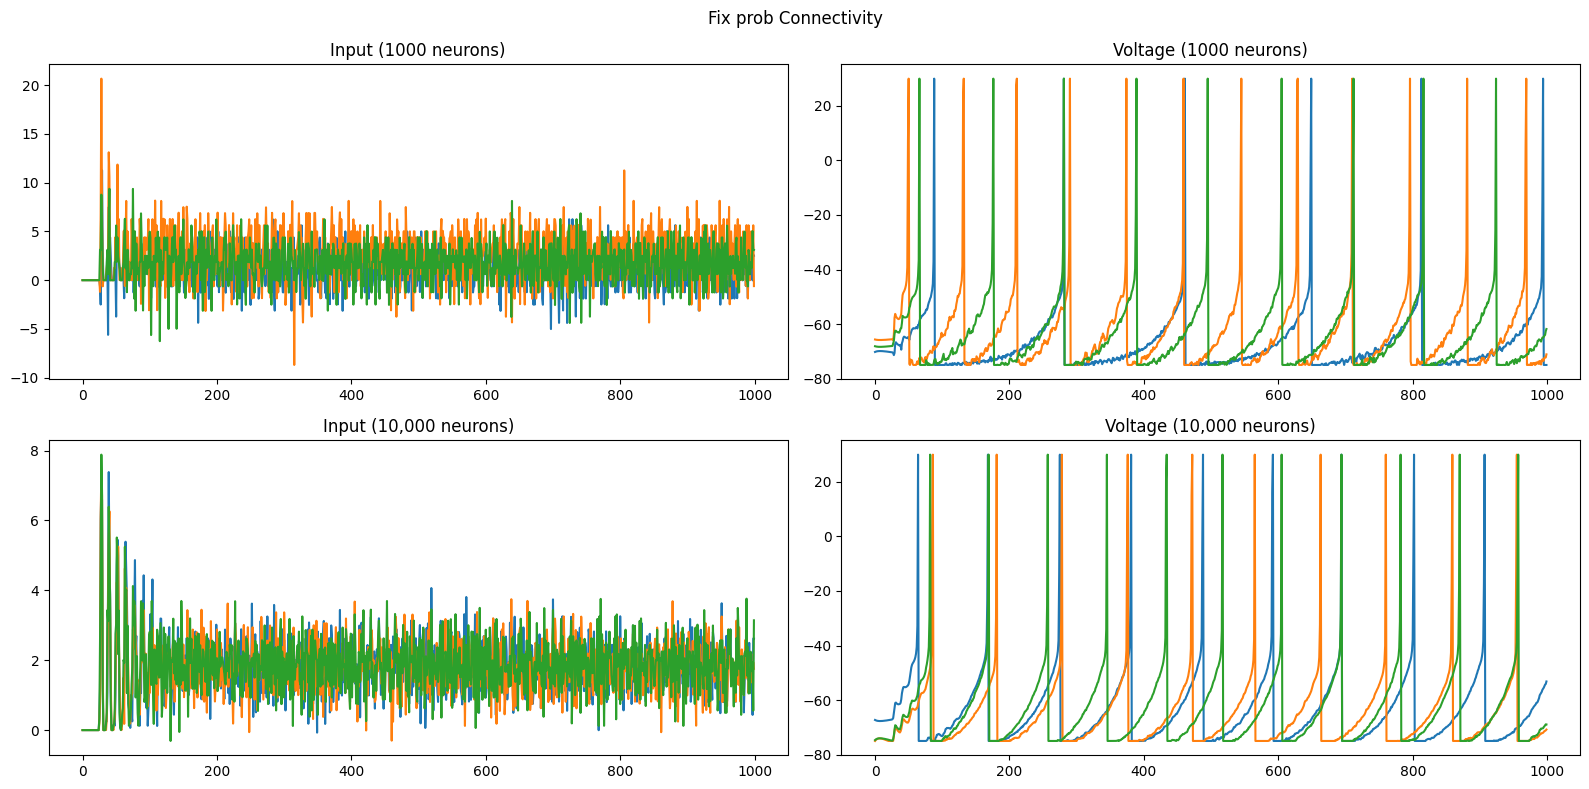
\includegraphics[width=1.2\textwidth]{fixProbCon.png}
		\caption{The model of fixed probability connectivity}
		\label{fixProb}
	\end{figure}
	
	\subsection{Fixed Number of Connections}
	To address the previous model pitfall, this is an alternative approach to keep a fixed number of pre-synaptic neurons for each post-synaptic ones. In this way, it does not matter how many possible connection exists, we always take a constant number. In our model, we take 10 neurons for this purpose.
	
	\begin{figure}[h]
		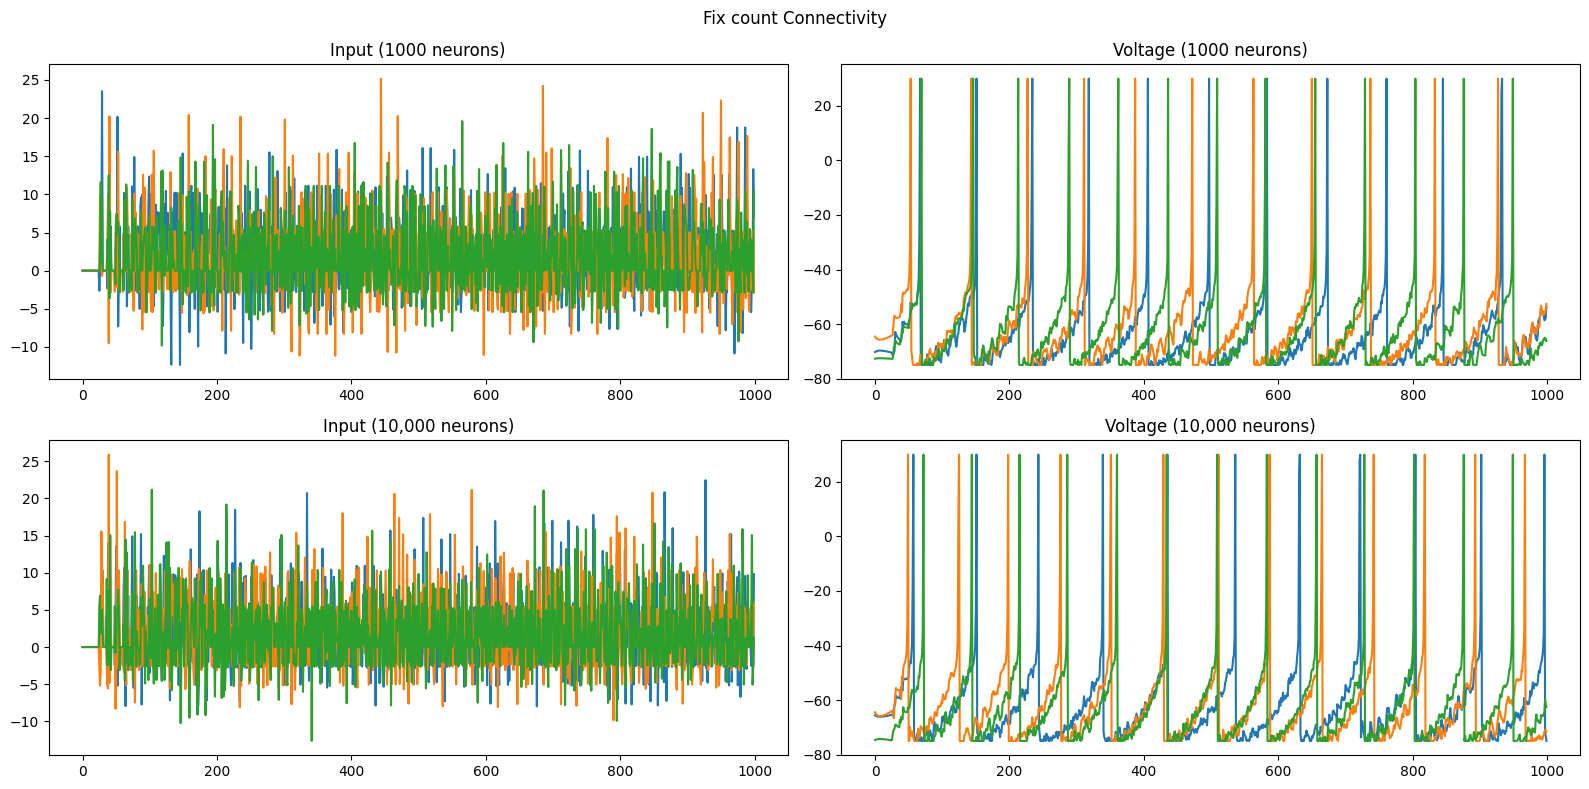
\includegraphics[width=1.2\textwidth]{fixCountCon.png}
		\caption{The model of fixed count connectivity}
		\label{fixCount}
	\end{figure}
	
	\subsection{Comparison}
	In all the three cases, as we increase the number of neurons, fluctuations decrease and we have a more robustness with 10,000 neurons.\\
	As in all cases the neural model is same, the key difference between these 3 connectivity patterns lies in their sensed input. In fully connected one, we had the least fluctuations, and it even lessened when we had a 10-fold scale-up. This phenomenon also happens in the second case, where the number of connections grows with the rate of neuron numbers growth.\\ However, as expected, this does not happen in the latter case. Because, the number of pre-synaptic neurons is independent of the total number of neurons.
	
	\section{Excite and Inhibit}
	Defined neural population are homogeneous. 
	\subsection{Part A}
	For this part, we created an excitatory and inhibitory population. The ratio of them is same as other parts ($\frac{\#exc}{\#inh} = \frac{1}{4}$), and there are a total of 1000 neurons. 
	
	\begin{figure}[h]
		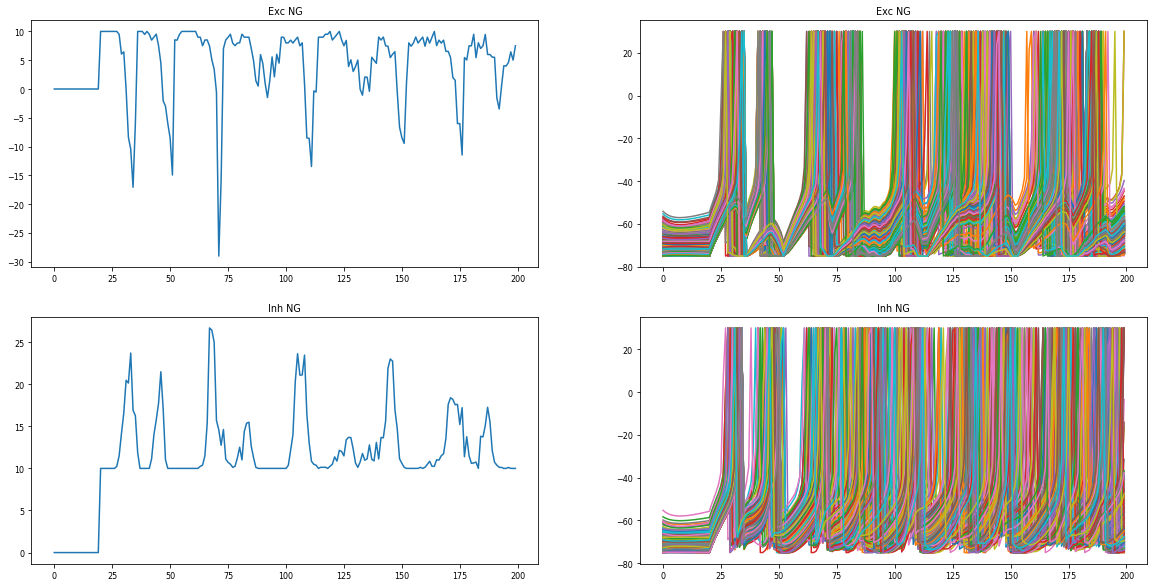
\includegraphics[width=1.2\textwidth]{input2.png}
		\caption{The input plots of the excitatory (top left plot) and inhibitory (bottom left plot) population. The corresponding voltages were shown in the right plots}
		\label{ei_inp}
	\end{figure}
	
	In figure \ref{ei_inp}, the aggregated input of each neuron groups were shown. Both the groups had a constant current of $10A$ in addition to their effect on each other. As the input of the inhibitory population increases, and the activity grows, it shows a proportional decrement in the input of the other population. \\
	
	The raster plot (figure \ref{raster1}) of these 2 population were shown, we can observe this effect more clearly. There is a periodic oscillation in the spikes, and after each spike peak in excitatory population, the inhibitory peak emerges. The activity of the populations is defined as the spikes count at each timestamp, which is visualized in the figure\ref{popAct}. Similarly, the inhibitory population activity growth after excitatory rise, and the inhibition of the bigger neuron group after inhibitory population is observable in the mentioned plot.\\
	
	
	\begin{figure}[h]
		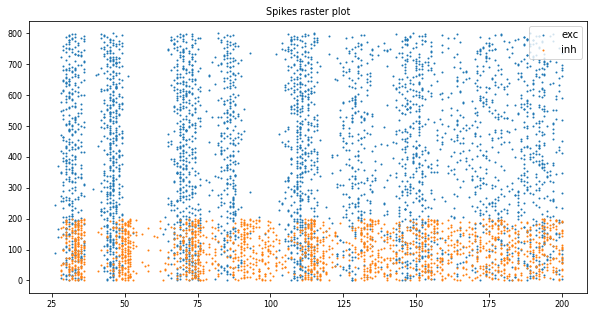
\includegraphics[width=\textwidth]{raster1.png}
		\caption{The raster plot of both population}
		\label{raster1}
	\end{figure}
	
	\begin{figure}[h]
		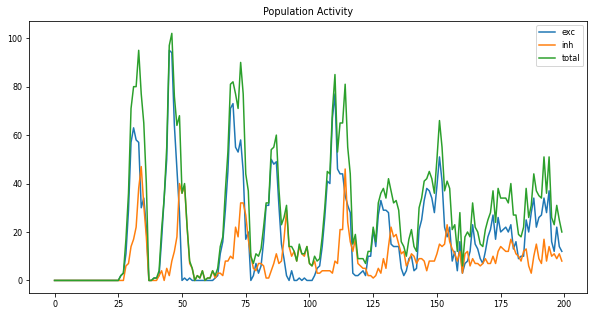
\includegraphics[width=\textwidth]{popAct.png}
		\caption{The populations activities}
		\label{popAct}
	\end{figure}
	
	\subsection{Part B}
	The previous plots were for delta synapse model where there was a full connectivity. For exploring how changing these parameters would change the population activity, we have plotted other connectivity patterns behavior.\\
	
	\begin{figure}[h]
		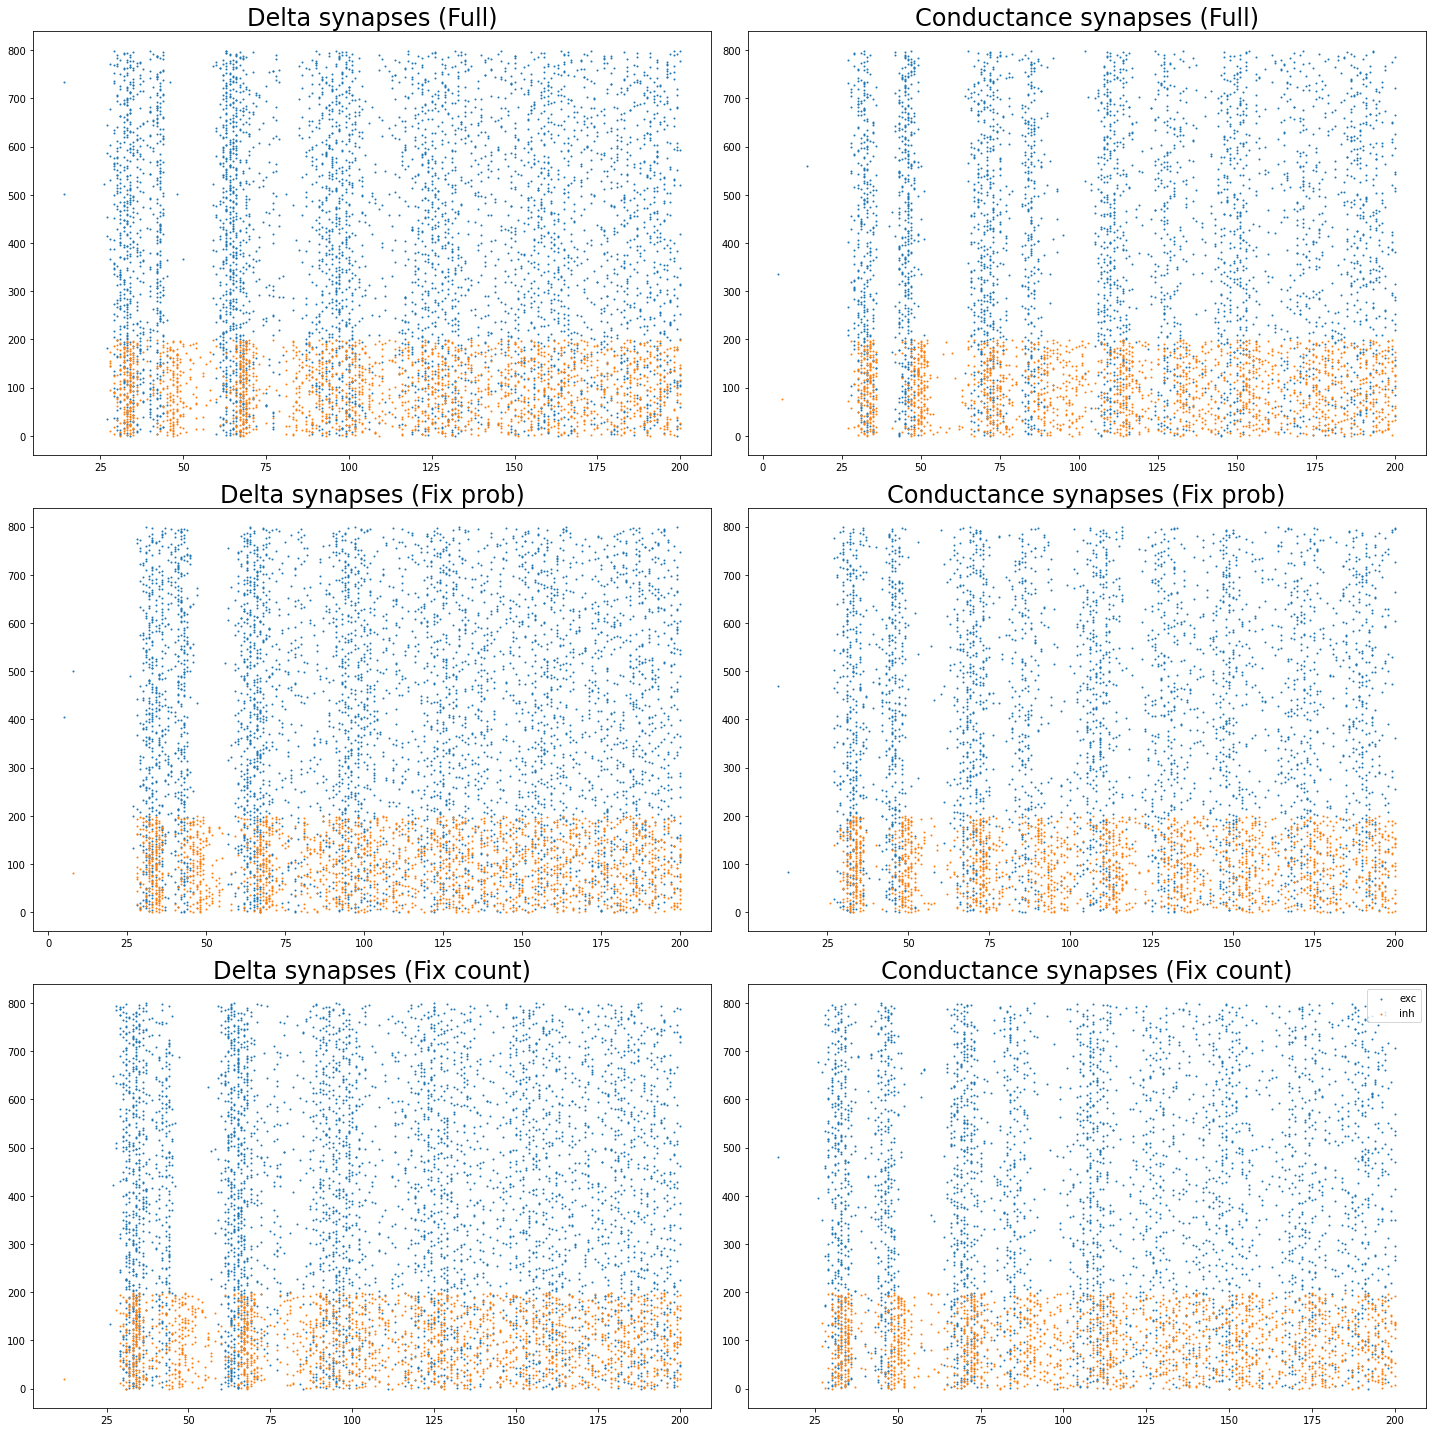
\includegraphics[width=1.2\textwidth]{raster2.png}
		\caption{Raster plots for different connectivity}
		\label{raster2}
	\end{figure}
	
	
	
\end{document}